\documentclass{article}

% Encodings, page setup, paragraph formatting, font
\usepackage[top=0.9in, bottom=1in, left=1.5in, right=1.5in]{geometry}
\usepackage[icelandic]{babel}
\usepackage[T1]{fontenc}
\usepackage[sc]{mathpazo}
\usepackage[parfill]{parskip}
\usepackage{cancel}
\usepackage{comment}
% Tables and lists
\usepackage{booktabs,tabularx}
\usepackage{multirow}
\usepackage{enumerate}
\usepackage{adjustbox}
\usepackage{multicol}
\usepackage{enumitem}
\usepackage{xcolor}
% Math
\usepackage{amsmath, amsfonts, amssymb, amsthm}
% Graphics
\usepackage{graphicx}
\usepackage{forest}
\usepackage{tikz}
\usetikzlibrary{positioning, shapes, arrows.meta}
% Code environment
\usepackage{listingsutf8}
\definecolor{commentcolor}{RGB}{0, 128, 0} % Grænn
\definecolor{keywordcolor}{RGB}{0, 0, 255}   % Blár
\definecolor{stringcolor}{RGB}{163, 21, 21}      % Dökkrauður
\definecolor{numbercolor}{RGB}{128, 0, 128}      % Fjólublár
\definecolor{identifiercolor}{RGB}{0, 0, 0}      % Svartur

\lstset{
    language=Java,
    basicstyle=\ttfamily,
    keywordstyle=\color{keywordcolor}\bfseries,
    commentstyle=\color{commentcolor},
    identifierstyle=\color{identifiercolor},
    stringstyle=\color{stringcolor},   
    showstringspaces=false,
    numbers=left,
    numberstyle=\tiny\color{gray},
    tabsize=2,
    breaklines=true,
    columns=fullflexible,
    keepspaces=true,
    inputencoding=utf8, 
    extendedchars=true,  
    literate=
        {á}{{\'a}}1
        {ð}{{\dh}}1
        {é}{{\'e}}1
        {í}{{\'i}}1
        {ó}{{\'o}}1
        {ú}{{\'u}}1
        {ý}{{\'y}}1
        {þ}{{\th}}1
        {æ}{{\ae}}1
        {ö}{{\"o}}1
        {Á}{{\'A}}1
        {Ð}{{\DH}}1
        {É}{{\'E}}1
        {Í}{{\'I}}1
        {Ó}{{\'O}}1
        {Ú}{{\'U}}1
        {Ý}{{\'Y}}1
        {Þ}{{\TH}}1
        {Æ}{{\AE}}1
        {Ö}{{\"O}}1,
}

% Restin af forskriftinni
\usepackage[pdftex,bookmarks=true,colorlinks=true,pdfauthor={Hafsteinn Einarsson},linkcolor=blue,urlcolor=blue]{hyperref}

% Hyphenation
\hyphenpenalty=5000
% Page and section numbering
\setcounter{secnumdepth}{-1} 
\pagenumbering{gobble}

\title{Tölvutækni og forritun Lokapróf}
\author{brj46 }
\date{Nóvember 2024}

\begin{document}

\maketitle

\vspace {7em}
\begin{center}
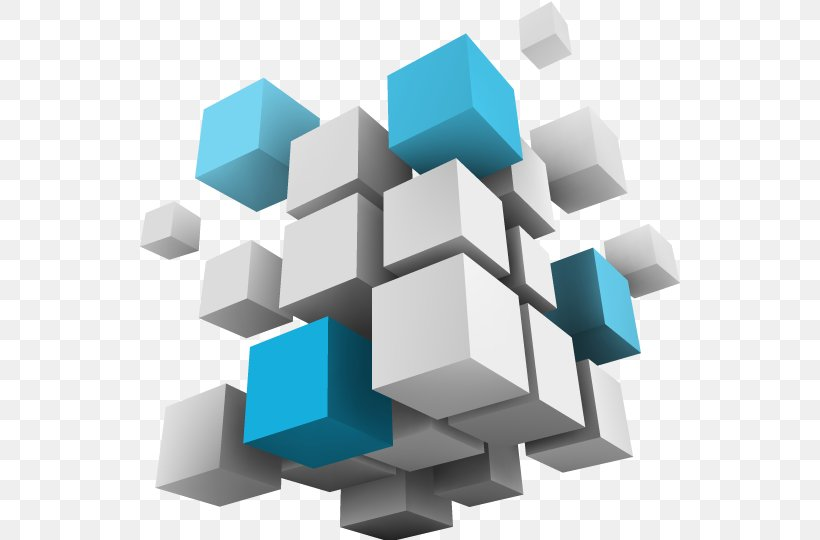
\includegraphics[width=0.7\textwidth]{3d.jpg}
\end{center}

\newpage
\section*{Hvað Þarf Ég Að Kunna?}

\begin{itemize}
    \item[$\square$] Varpanir (tvívíðar og þrívíðar) (töluleg rök)
    \item[$\square$] Hreyfanleg líkön (WebGl) (Render-Föll)
    \item[$\square$] Endurskinslíkön (Phong lýsingarlíkanið) (útreikningar með dofnun)
    \item[$\square$] Mynsturvörpun (Texture mapping t.d. repeat og \text{CLAMP\_TO\_EDGE}) Ójafnhliða síun
    \item[$\square$] GLSL og litaraforritun (Hnúta- og bútalitarar) (Hreyfing og litabreytingar)
    \item[$\square$] Ýmis atriði í tölvugrafík (Homogeneous hnit) (þríhyrnaröðun)(Skuggakort)
    \item[$\square$] Aukaverkefni (Geislasmölun vs Phong) (Dofnun og birtustýring)
\end{itemize}

\end{document}